In the search for new physics signal it may happen that the experiment does not
have the sensitivity to exclude a particular model. This can happen for example
when testing the hypothesis of some \gls{susy} particles with a mass greater
than what can be produced at \gls{lhc}. In this case the frequentist approach
described in \cref{sec:stat-proc} for setting upper exclusion limits when
$p_\mu < \alpha$ will reject the model with a probability of $\alpha$ or
greater~\cite{CowanCLsPlots}. In general this kind of situation happens whenever
the signal plus background distribution is very similar to the background only
one.

The $\cls$ method~\cite{CLsMethod} can be used in such situations. This more
conservative method prevents the rejection of models where the sensitivity is
low reverting to the frequentist procedure introduced in \cref{sec:stat-proc}
for models with higher sensitivity. The method defines the quantity:
\begin{equation}
  \label{eq:126}
  \cls = \frac{p_{s + b}}{1 - p_b}
\end{equation}
where $p_{s + b}$ and $p_b$ correspond to the p-value for the signal plus
background ($\mu = 0$) and background only ($\mu = 0$) hypothesis
respectively. The $\cls$ value is then used in place of the p-value and the
inequality $\cls \leq \alpha$ is evaluated
instead. \cref{fig:cls_underfluctuation} allows to understand qualitatively how
the method works, in the figure the test statistics $Q$ is similar both for the
signal plus background and for the background only hypotheses. If
$Q_\mathrm{obs}$ is such that $p_{s + b} < \alpha$, in the frequentist approach
described in \cref{sec:stat-proc} the signal plus background hypothesis would be
rejected while using the $\cls$ method it is possible to see that, since $p_b$
is big and thus $1 - p_b$ is small, the ratio in \cref{eq:126} will be greater
than $p_{s + b}$ and the model is not rejected. In the case of high sensitivity,
the signal plus background and the background only hypothesis distributions are
well separated as depicted in \cref{fig:cls_ingredients}. In this case if
$Q_\mathrm{obs}$ is such that $p_{s + b} < \alpha$ then $p_b$ is small and,
being the denominator in \cref{eq:126} close to one, the $\cls$ method becomes
similar to the usual frequentist approach of \cref{sec:stat-proc} where the
p-value $p_{s + b}$ is tested~\cite{CLsMethod}.
\begin{figure}[!h]
  \centering
  \begin{subfigure}{.48\linewidth}
    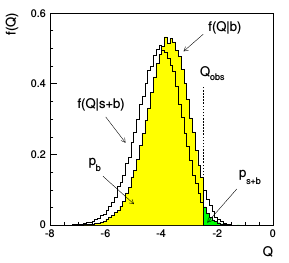
\includegraphics[width=\linewidth]{cls_underfluctuation}
    \caption{Low sensitivity to new signal.}
    \label{fig:cls_underfluctuation}
  \end{subfigure}
  \begin{subfigure}{.48\linewidth}
    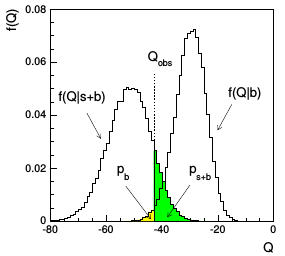
\includegraphics[width=\linewidth]{cls_ingredients}
    \caption{High sensitivity to new signal.}
    \label{fig:cls_ingredients}
  \end{subfigure}
  \caption{Graphical illustration of the $\cls$ method. In
    \cref{fig:cls_underfluctuation} the low sensitivity would lead to the
    rejection of the $p_{s + b}$ hypothesis if the $\cls$ method is not
    used. In the case of two well separated distributions like in
    \cref{fig:cls_ingredients} the use of the $\cls$ method is equivalent to the
    usual frequentist approach~\cite{CowanCLsPlots}.}
  \label{fig:cls_method}
\end{figure}
%%% Local Variables:
%%% mode: latex
%%% TeX-master: "../search_for_DM_LED_with_ATLAS"
%%% End:
